\chapter{心脏与心动周期}\label{ch:b2:heart}

取出一只青蛙\omterm{def:b2:heart:anatomy}{心脏}，放入盐溶液中，它仍会
持续跳动数小时——没有神经，没有脑，没有\omterm{def:b2:blood-circulation:blood}{血液}，
只是一块肌肉，因其局部一小片细胞无法保持静止，
每秒约自行收缩一次。人的\omterm{def:b2:heart:anatomy}{心脏}一生中约跳动
三十亿次，泵出约两亿升\omterm{def:b2:blood-circulation:blood}{血液}，且从不停止。
本章讨论这台泵：它的腔室与瓣膜，充盈与排空的循环，
驱动循环的压强，控制其节律的电系统，
以及它在皮肤上留下的电痕迹，
使其输出量逐搏与流入量相匹配的规律，
以及神经和激素，
它们调节\omterm{def:b2:heart:anatomy}{心脏}的搏动频率与收缩力。

\section{泵}

\begin{definition}[腔室与瓣膜]\label{def:b2:heart:anatomy}
\index{心脏}\index{心房}\index{心室}\index{心脏瓣膜}
心脏是两台并列的泵，每台都包括一个从\omterm{def:b2:blood-circulation:vessels}{静脉}接收\omterm{def:b2:blood-circulation:blood}{血液}的\emph{心房}，
以及一个将\omterm{def:b2:blood-circulation:blood}{血液}射入\omterm{def:b2:blood-circulation:vessels}{动脉}的\emph{心室}。右心从腔\omterm{def:b2:blood-circulation:vessels}{静脉}接收\omterm{def:b2:blood-circulation:blood}{血液}，
经肺\omterm{def:b2:blood-circulation:vessels}{动脉}将其送至肺；左心从肺\omterm{def:b2:blood-circulation:vessels}{静脉}接收\omterm{def:b2:blood-circulation:blood}{血液}，
经主\omterm{def:b2:blood-circulation:vessels}{动脉}将其送至全身。四个瓣膜保证血流单向流动，
分为两类：
其一为
\emph{房室瓣}（右侧为三尖瓣，左侧为二尖瓣），
瓣叶由腱索系于乳头肌上，使其不致被推回心房；
其二为
\emph{半月瓣}（肺\omterm{def:b2:blood-circulation:vessels}{动脉}瓣与主\omterm{def:b2:blood-circulation:vessels}{动脉}瓣），
由三个袋状瓣叶组成，\omterm{def:b2:blood-circulation:vessels}{动脉}压超过心室压时充盈闭合。
瓣膜是被动的：仅凭压差即可开启与关闭。
心室壁是\emph{心肌}，
为横纹肌，由分支细胞首尾相接而成，
细胞间借\emph{闰盘}相连，闰盘内充满缝隙连接，使整个心室在电学上如同一个细胞，
整体同步收缩；左心室壁厚度约为右心室的三倍，
因其所对抗的压强约为右心室的五倍。
心肌由其自身的
\emph{冠状\omterm{def:b2:blood-circulation:vessels}{动脉}}供血，这些\omterm{def:b2:blood-circulation:vessels}{动脉}在\omterm{prop:b2:heart:cycle}{舒张期}充盈，
心肌几乎完全依赖有氧代谢，无法“借贷”能量。
\end{definition}

\begin{omfigure}
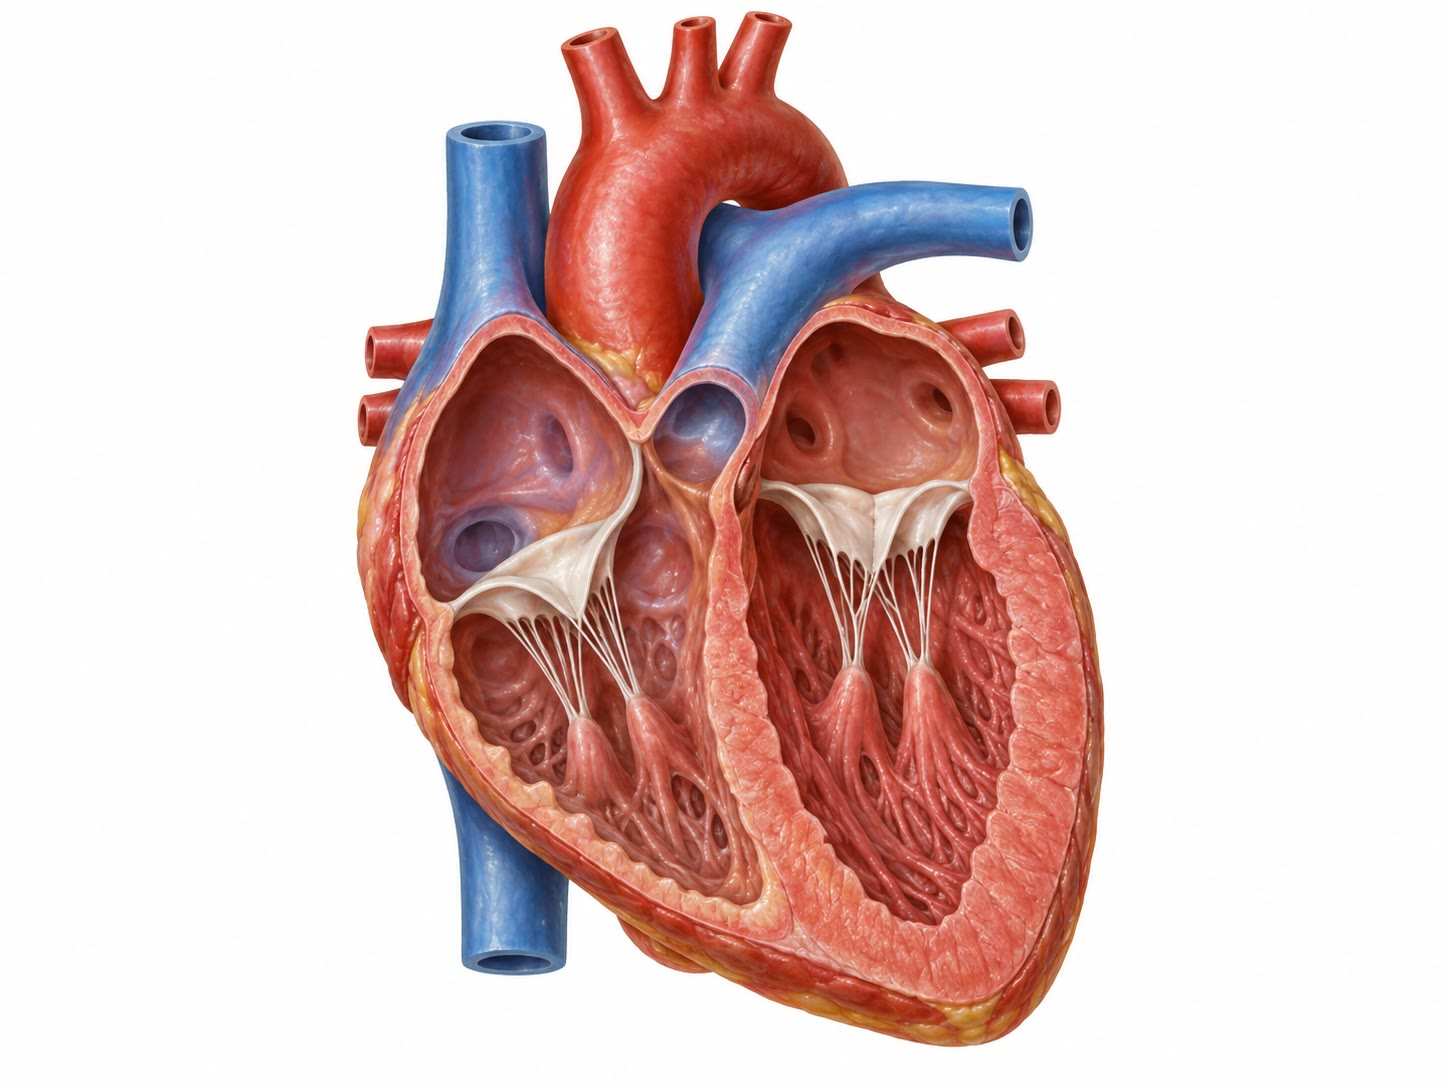
\includegraphics[width=0.55\linewidth]{images/book4/ai/b4-17-heart-cutaway.jpg}

{\small \omterm{def:b2:heart:anatomy}{心脏}正面剖面：上方为两个\omterm{def:b2:heart:anatomy}{心房}，下方为两个\omterm{def:b2:heart:anatomy}{心室}，
左\omterm{def:b2:heart:anatomy}{心室}壁较厚，房室瓣及其腱索，
顶部为两条大\omterm{def:b2:blood-circulation:vessels}{动脉}射出。}
\end{omfigure}

\begin{proposition}[心动周期]\label{prop:b2:heart:cycle}
\index{心动周期}\index{收缩期}\index{舒张期}\index{每搏输出量}\index{射血分数}
静息时一次搏动约持续 \qty{0.8}{s}。\emph{\omterm{prop:b2:heart:cycle}{舒张期}}
（\qty{0.5}{s}）：\omterm{def:b2:heart:anatomy}{心室}舒张，压强降至低于\omterm{def:b2:heart:anatomy}{心房}压，房室瓣开启，\omterm{def:b2:blood-circulation:blood}{血液}流入，
其中大部分为被动充盈，
随后由\omterm{def:b2:heart:anatomy}{心房}收缩给予最后一次推动；
舒张末期\omterm{def:b2:heart:anatomy}{心室}内约含 \qty{120}{mL} \omterm{def:b2:blood-circulation:blood}{血液}（即
\emph{舒张末期容积}）。\emph{\omterm{prop:b2:heart:cycle}{收缩期}}（\qty{0.3}{s}）：\omterm{def:b2:heart:anatomy}{心室}
收缩；一旦其压强超过\omterm{def:b2:heart:anatomy}{心房}压，
房室瓣即闭合（产生第一心音，即“噗”音），
随后，\omterm{def:b2:heart:anatomy}{心室}在数百分之一秒内挤压一个封闭的腔室，
即\emph{等容收缩}，直至其压强超过\omterm{def:b2:blood-circulation:vessels}{动脉}压，
左侧\omterm{def:b2:blood-circulation:vessels}{动脉}压为 \qty{80}{mmHg}，
此时半月瓣开启，\omterm{def:b2:blood-circulation:blood}{血液}被射出。
左\omterm{def:b2:heart:anatomy}{心室}压强升至 \qty{120}{mmHg}，射出约
\qty{70}{mL} \omterm{def:b2:blood-circulation:blood}{血液}（即\emph{\omterm{prop:b2:heart:cycle}{每搏输出量}}，其\emph{\omterm{prop:b2:heart:cycle}{射血分数}}为 \qty{60}{\%}）；
\omterm{def:b2:heart:anatomy}{心室}舒张时，压强降至低于主\omterm{def:b2:blood-circulation:vessels}{动脉}压，
主\omterm{def:b2:blood-circulation:vessels}{动脉}瓣迅速关闭（产生第二心音，即“咚”音），
随后经等容舒张使压强降至\omterm{def:b2:heart:anatomy}{心房}水平，充盈随即恢复。
右心的过程相同，压强约为左心的五分之一，
射出的血量相同。
\end{proposition}

\begin{omfigure}
\begin{tikzpicture}
\begin{axis}[
  width=0.9\linewidth, height=7.2cm,
  axis x line=bottom, axis y line=left,
  xmin=0, xmax=0.8, ymin=0, ymax=130,
  xlabel={心动周期中的时间 (s)}, ylabel={压强 (\unit{mmHg})},
  xlabel style={font=\small, at={(axis description cs:0.5,-0.1)}, anchor=north},
  ylabel style={font=\small},
  tick label style={font=\small}, xtick={0,0.1,0.3,0.8}, ytick={0,40,80,120},
  legend style={font=\scriptsize, at={(0.6,0.45)}, anchor=west, draw=none},
  clip=false,
]
% aortic pressure
\addplot[very thick, omThm] coordinates {(0,82) (0.05,80) (0.1,80) (0.12,95) (0.16,115) (0.2,120) (0.25,112) (0.3,100) (0.32,104) (0.34,100) (0.45,94) (0.6,88) (0.8,82)};
\addlegendentry{主动脉}
% left ventricular pressure
\addplot[very thick, omDef] coordinates {(0,5) (0.04,8) (0.05,10) (0.08,60) (0.1,80) (0.12,95) (0.16,115) (0.2,120) (0.25,112) (0.3,100) (0.32,60) (0.35,20) (0.38,5) (0.5,3) (0.7,5) (0.75,8) (0.8,5)};
\addlegendentry{左心室}
% atrial pressure
\addplot[thick, omProp] coordinates {(0,6) (0.03,9) (0.06,6) (0.1,8) (0.15,6) (0.3,7) (0.36,10) (0.4,5) (0.6,6) (0.75,9) (0.8,6)};
\addlegendentry{左心房}
\draw[dashed, gray] (axis cs:0.05,0) -- (axis cs:0.05,128); \node[font=\scriptsize, anchor=south, align=center] at (axis cs:0.05,128) {二尖瓣 \\闭合};
\draw[dashed, gray] (axis cs:0.1,0) -- (axis cs:0.1,128); \node[font=\scriptsize, anchor=south, align=center] at (axis cs:0.13,128) {主动脉瓣 \\开启};
\draw[dashed, gray] (axis cs:0.31,0) -- (axis cs:0.31,128); \node[font=\scriptsize, anchor=south, align=center] at (axis cs:0.31,128) {主动脉瓣 \\闭合};
\draw[dashed, gray] (axis cs:0.38,0) -- (axis cs:0.38,128); \node[font=\scriptsize, anchor=south, align=center] at (axis cs:0.4,128) {二尖瓣 \\开启};
\node[font=\scriptsize] at (axis cs:0.2,45) {收缩期};
\node[font=\scriptsize] at (axis cs:0.55,25) {舒张期};
\end{axis}
\end{tikzpicture}

{\small 左心在一次搏动中的压强变化。\omterm{def:b2:heart:anatomy}{心室}
在封闭腔室中收缩，直至压强超过主\omterm{def:b2:blood-circulation:vessels}{动脉}压；
压强高于主\omterm{def:b2:blood-circulation:vessels}{动脉}压时射血，随后舒张，直至压强降至\omterm{def:b2:heart:anatomy}{心房}压以下；
随后充盈。}
\end{omfigure}

\begin{theorem}[心脏的做功]\label{thm:b2:heart:work}
\index{心脏做功}\index{压强–容积环}
以压强对容积作图，左\omterm{def:b2:heart:anatomy}{心室}的一次搏动描出一个
环：沿下缘为充盈，
沿右侧为等容收缩，沿上缘为射血，
从 \qty{120}{mL} 降至 \qty{50}{mL}，沿左侧为等容舒张，
该环的面积即为一次搏动的
机械功：
\[
W = \oint P\,\mathrm{d}V \approx \bar P_{\text{射血}}\times \text{每搏输出量} \approx \qty{100}{mmHg}\times\qty{70}{mL} = \qty{0.93}{J}.
\]
以每分钟 72 次计，左\omterm{def:b2:heart:anatomy}{心室}做功约 \qty{1.1}{W}，
右\omterm{def:b2:heart:anatomy}{心室}约 \qty{0.2}{W}；\omterm{def:b2:heart:anatomy}{心脏}的代谢功率约为 \qty{8}{W}，因此其
机械效率接近 \qty{15}{\%}，其余能量转化为热量
及张力所耗的能量。提高\omterm{def:b2:heart:anatomy}{心脏}泵血所对抗的压强
（如高血压、主\omterm{def:b2:blood-circulation:vessels}{动脉}瓣狭窄）会使每搏做功按比例增加，
心肌亦随之增厚，与任何肌肉的反应一致——
直至其冠状\omterm{def:b2:blood-circulation:vessels}{动脉}供血已无法跟上肌肉的增大。
\end{theorem}
\begin{proof}
功等于力乘以距离；对于作用在运动
壁面上的压强，其功为压强乘以扫过的容积：$\mathrm{d}W = P\,\mathrm{d}V$。
沿封闭回路做功的净值即为所围面积（充盈时压强低，耗能很少；
射血时压强高，返还较多）。
$\qty{100}{mmHg} = \qty{1.33e4}{Pa}$ 和 $\qty{70}{mL} =
\qty{7e-5}{m^3}$：$1.33\times 10^{4}\times 7\times 10^{-5} =
\qty{0.93}{J}$；乘以每秒 $1.2$ 次搏动，得 \qty{1.1}{W}。
\end{proof}

\begin{omfigure}
\begin{tikzpicture}
\begin{axis}[
  width=0.62\linewidth, height=6cm,
  axis x line=bottom, axis y line=left,
  xmin=0, xmax=150, ymin=0, ymax=140,
  xlabel={左心室容积（\unit{mL}）}, ylabel={压强（\unit{mmHg}）},
  xlabel style={font=\small, at={(axis description cs:0.5,-0.12)}, anchor=north},
  ylabel style={font=\small},
  tick label style={font=\small}, xtick={0,50,120}, ytick={0,80,120},
  clip=false,
]
\fill[omDef!12] (axis cs:50,5) -- (axis cs:120,8) -- (axis cs:120,80) -- (axis cs:110,115) -- (axis cs:80,122) -- (axis cs:50,100) -- cycle;
\draw[very thick, omDef, ->] (axis cs:50,5) -- (axis cs:120,8);
\draw[very thick, omDef, ->] (axis cs:120,8) -- (axis cs:120,80);
\draw[very thick, omDef, ->] (axis cs:120,80) .. controls (axis cs:110,118) and (axis cs:80,125) .. (axis cs:50,100);
\draw[very thick, omDef, ->] (axis cs:50,100) -- (axis cs:50,5);
\node[font=\scriptsize, anchor=south] at (axis cs:85,11) {充盈};
\node[font=\scriptsize, anchor=west] at (axis cs:122,44) {等容收缩};
\node[font=\scriptsize, anchor=south] at (axis cs:85,124) {射血};
\node[font=\scriptsize, anchor=east] at (axis cs:48,52) {舒张};
\node[font=\scriptsize] at (axis cs:85,60) {面积 $=$ 功，\qty{0.9}{J}};
\end{axis}
\end{tikzpicture}

{\small 左\omterm{def:b2:heart:anatomy}{心室}的压力–容积环。所围面积即为一次搏动的功；
\omterm{def:b2:blood-circulation:vessels}{动脉}压升高会抬高
环的上缘，功也随之增大。}
\end{omfigure}

\section{心脏自身的节律}

\begin{proposition}[自动节律与传导]\label{prop:b2:heart:conduction}
\index{窦房结}\index{起搏点}\index{房室结}\index{浦肯野纤维}
搏动起源于\emph{\omterm{prop:b2:heart:conduction}{窦房结}}，这是一小片
位于右\omterm{def:b2:heart:anatomy}{心房}壁内的特化肌细胞，其
膜电位从不静息：每次动作电位之后，它
会缓慢上升（即\emph{起搏电位}，由
在负电位时开启的钠电流和
钙通道驱动），直至达到阈值并再次放电，若不受干扰，约
每分钟一百次。冲动沿\omterm{def:b2:heart:anatomy}{心房}肌扩散，
细胞间经缝隙连接逐个传递，\omterm{def:b2:heart:anatomy}{心房}随之收缩；
随后冲动到达\emph{\omterm{prop:b2:heart:conduction}{房室结}}，它是
\omterm{def:b2:heart:anatomy}{心房}与\omterm{def:b2:heart:anatomy}{心室}之间唯一的电联系，传导缓慢，
使冲动延迟约十分之一秒，为\omterm{def:b2:heart:anatomy}{心房}
完成对\omterm{def:b2:heart:anatomy}{心室}的充盈留出时间；随后冲动沿
\emph{希氏束}和\emph{\omterm{prop:b2:heart:conduction}{浦肯野纤维}}迅速下传，
后者为传导很快的细胞，可在
\qty{30}{ms} 内将冲动送达整个\omterm{def:b2:heart:anatomy}{心室}肌，使\omterm{def:b2:heart:anatomy}{心室}自心尖向上
作为一个整体收缩，把\omterm{def:b2:blood-circulation:blood}{血液}推向流出道瓣膜。
这一系统的每个部分都能自行起搏，但频率依次递减
（\omterm{prop:b2:heart:conduction}{窦房结} 100，\omterm{prop:b2:heart:conduction}{房室结} 50，\omterm{prop:b2:heart:conduction}{浦肯野纤维} 30），
因此若\omterm{prop:b2:heart:conduction}{窦房结}失灵，较低位的中心便会接管，
只是节律更慢。
\end{proposition}
\begin{proof}[证据]
离体\omterm{def:b2:heart:anatomy}{心脏}或一条窦房组织，在培养皿中仍能搏动，
无需神经；一条\omterm{def:b2:heart:anatomy}{心室}肌条也能搏动，但更慢。
单独降温或升温\omterm{prop:b2:heart:conduction}{窦房结}，会改变整个\omterm{def:b2:heart:anatomy}{心脏}的节律；
切断房室束，\omterm{def:b2:heart:anatomy}{心室}与\omterm{def:b2:heart:anatomy}{心房}分离，
\omterm{def:b2:heart:anatomy}{心室}便以其自身较慢的节律搏动，而\omterm{def:b2:heart:anatomy}{心房}
仍按\omterm{prop:b2:heart:conduction}{窦房结}的节律运行（\omterm{def:b2:heart:anatomy}{心脏}传导阻滞）。记录单个\omterm{prop:b2:heart:conduction}{窦房结}细胞，
可见一种缓慢的\omterm{prop:b2:heart:cycle}{舒张期}去极化，这是一般肌细胞所没有的；
阻断起搏电流则使其减慢。
\end{proof}

\begin{omfigure}
\begin{tikzpicture}[every node/.style={font=\scriptsize}, >=stealth]
  % simplified heart outline, scaled up
  \draw[thick, fill=omThm!6] (0,0) .. controls (-4.2,1.3) and (-3.8,5.4) .. (-1.3,5.8) .. controls (0,6.1) and (0.6,5.6) .. (1.3,5.8) .. controls (3.8,5.4) and (4.2,1.3) .. (0,0);
  \draw[thick] (-3.0,3.5) .. controls (-0.8,3.85) and (0.8,3.85) .. (3.0,3.5);
  \draw[thick] (0,3.75) -- (0,0.6);
  \node at (-1.5,4.7) {右心房}; \node at (1.5,4.7) {左心房};
  \node[align=center] at (-1.3,2.55) {右 \\心室}; \node[align=center] at (1.3,2.55) {左 \\心室};
  % SA node
  \fill[omDef] (-2.5,5.0) circle (0.16); \node[omDef, anchor=east] at (-3.3,5.4) {窦房结}; \draw[omDef] (-3.3,5.35) -- (-2.62,5.08);
  \draw[omDef, dashed] (-2.5,5.0) circle (0.45); \draw[omDef, dashed] (-2.5,5.0) circle (0.8);
  % AV node
  \fill[omDef] (-0.25,3.7) circle (0.14); \node[omDef, anchor=west] at (0.15,4.05) {房室结}; \draw[omDef] (0.15,4.05) -- (-0.12,3.78);
  % bundle and Purkinje
  \draw[very thick, omDef] (-0.25,3.6) -- (-0.25,2.1);
  \draw[very thick, omDef] (-0.25,2.1) .. controls (-0.8,1.4) .. (-1.9,1.1);
  \draw[very thick, omDef] (-0.25,2.1) .. controls (0.8,1.4) .. (1.9,1.1);
  \foreach \p in {(-1.9,1.1),(1.9,1.1)} { \draw[omDef] \p -- ++(-0.3,0.6); \draw[omDef] \p -- ++(0.3,0.7); \draw[omDef] \p -- ++(0,0.85); }
  \node[omDef, anchor=west] at (3.4,1.0) {浦肯野纤维}; \draw[omDef] (3.4,1.0) -- (2.2,1.1);
  \node[omDef, anchor=east] at (-0.45,3.05) {希氏束};
  % timing
  \node[anchor=west, align=left] at (5.6,5.0) {窦房结发放：$t = 0$\\心房去极化：0--\qty{80}{ms}};
  \node[anchor=west, align=left] at (5.6,3.5) {房室结延迟：\qty{100}{ms}};
  \node[anchor=west, align=left] at (5.6,1.9) {希氏束与浦肯野纤维：\\心室去极化 \\在 \qty{220}{ms} 时完成，自心尖开始};
\end{tikzpicture}

{\small 传导系统。\omterm{prop:b2:heart:conduction}{窦房结}发放冲动，\omterm{def:b2:heart:anatomy}{心房}去极化，
\omterm{prop:b2:heart:conduction}{房室结}延迟冲动，
希氏束与\omterm{prop:b2:heart:conduction}{浦肯野纤维}
自心尖向上将冲动送至\omterm{def:b2:heart:anatomy}{心室}。}
\end{omfigure}

\begin{proposition}[心电图]\label{prop:b2:heart:ecg}
\index{心电图}
\omterm{def:b2:heart:anatomy}{心脏}是由大量细胞依次去极化、复极化构成的大团块，
其周围体内流动的电流，可在四肢上的电极之间记录为毫伏级电压，即\emph{\omterm{prop:b2:heart:ecg}{心电图}}。
其波形对应传导系统中的各个事件：\emph{P 波}为\omterm{def:b2:heart:anatomy}{心房}去极化；
平坦的\emph{PR 间期}（\qty{0.16}{s}）为房室延迟；
尖锐而短暂的\emph{QRS 波群}（\qty{0.08}{s}）为\omterm{def:b2:heart:anatomy}{心室}去极化，
幅度大是因为\omterm{def:b2:heart:anatomy}{心室}质量大，
持续时间短是因为\omterm{prop:b2:heart:conduction}{浦肯野纤维}传导快；\emph{T 波}为\omterm{def:b2:heart:anatomy}{心室}复极化。
（\omterm{def:b2:heart:anatomy}{心房}复极化被埋没在 QRS 中。）
\omterm{prop:b2:heart:ecg}{心电图}反映的是时序与传导，而非收缩力：
\omterm{prop:b2:heart:conduction}{房室结}受阻会延长 PR 间期，
或使 P 波与 QRS 分离；
\omterm{def:b2:heart:anatomy}{心室}的一段失活区会使 QRS 变形；
\omterm{def:b2:heart:anatomy}{心房}不规则（\omterm{def:b2:heart:anatomy}{心房}颤动）会以杂乱波形取代 P 波，
并使\omterm{def:b2:heart:anatomy}{心室}搏动不规则；
R 波之间的间隔则可用来求得心率。
\end{proposition}

\begin{omfigure}
\begin{tikzpicture}
\begin{axis}[
  width=0.9\linewidth, height=5.2cm,
  axis x line=bottom, axis y line=left,
  xmin=0, xmax=1.0, ymin=-0.4, ymax=1.3,
  xlabel={时间 (s)}, ylabel={mV},
  xlabel style={font=\small, at={(axis description cs:0.5,-0.12)}, anchor=north},
  ylabel style={font=\small},
  tick label style={font=\small}, xtick={0,0.2,0.4,0.6,0.8,1.0}, ytick={0,1},
  clip=false,
]
\addplot[very thick, omDef] coordinates {(0,0) (0.08,0) (0.1,0.05) (0.14,0.15) (0.18,0.05) (0.2,0) (0.28,0) (0.3,-0.1) (0.31,0) (0.33,1.1) (0.35,0) (0.36,-0.25) (0.375,0) (0.5,0) (0.54,0.1) (0.58,0.28) (0.62,0.1) (0.65,0) (0.88,0) (0.9,0.05) (0.94,0.15) (0.98,0.05) (1.0,0)};
\node[font=\scriptsize, anchor=south] at (axis cs:0.14,0.17) {P};
\node[font=\scriptsize, anchor=south] at (axis cs:0.33,1.12) {R};
\node[font=\scriptsize, anchor=north] at (axis cs:0.295,-0.11) {Q};
\node[font=\scriptsize, anchor=north] at (axis cs:0.365,-0.27) {S};
\node[font=\scriptsize, anchor=south] at (axis cs:0.58,0.3) {T};
\draw[<->, gray] (axis cs:0.1,0.45) -- (axis cs:0.3,0.45); \node[font=\scriptsize, anchor=south, gray] at (axis cs:0.2,0.46) {PR \qty{0.16}{s}};
\draw[<->, gray] (axis cs:0.3,0.6) -- (axis cs:0.375,0.6); \node[font=\scriptsize, anchor=west, gray] at (axis cs:0.38,0.6) {QRS \qty{0.08}{s}};
\draw[<->, gray] (axis cs:0.33,1.25) -- (axis cs:0.94,1.25); \node[font=\scriptsize, anchor=south, gray] at (axis cs:0.63,1.25) {R--R 间期 $=$ 60/速率};
\end{axis}
\end{tikzpicture}

{\small 正常\omterm{prop:b2:heart:ecg}{心电图}：P（\omterm{def:b2:heart:anatomy}{心房}）、\omterm{prop:b2:heart:conduction}{房室结}处的
PR 延迟、QRS（\omterm{def:b2:heart:anatomy}{心室}去极化）、
T（\omterm{def:b2:heart:anatomy}{心室}复极化）。}
\end{omfigure}

\section{调节输出}

\begin{theorem}[弗兰克–斯塔林定律]\label{thm:b2:heart:starling}
\index{弗兰克–斯塔林定律}\index{前负荷}\index{心输出量}
\omterm{def:b2:heart:anatomy}{心室}收缩的力随充盈它的容积增大而增大：在工作范围内，
\omterm{prop:b2:heart:cycle}{舒张期}\omterm{def:b2:heart:anatomy}{心室}被拉伸得越多（\emph{\omterm{thm:b2:heart:starling}{前负荷}}），\omterm{prop:b2:heart:cycle}{收缩期}
射出的\omterm{def:b2:blood-circulation:blood}{血液}就越多。因此\omterm{def:b2:heart:anatomy}{心脏}逐搏泵出它所接收的全部\omterm{def:b2:blood-circulation:blood}{血液}——
\omterm{def:b2:blood-circulation:vessels}{静脉}回流增加 \qty{20}{\%}，
\omterm{prop:b2:heart:cycle}{每搏输出量}便随之增加 \qty{20}{\%}，
无需神经或激素参与——
而左右两\omterm{def:b2:heart:anatomy}{心室}必须输送等量\omterm{def:b2:blood-circulation:blood}{血液}，
它们会自动达成平衡：
若右心向肺部输送的\omterm{def:b2:blood-circulation:blood}{血液}增多，
左心接收的\omterm{def:b2:blood-circulation:blood}{血液}也随之增多，泵出量亦增。
其机制在于\omterm{def:b2:cell-differentiation:fibre}{肌节}：充盈不足的\omterm{def:b2:heart:anatomy}{心室}
处于较短长度时，粗、细肌丝重叠过多，
钙敏感性低；拉伸至最适长度（\qty{2.2}{\micro m}）时，
可供横桥结合的重叠增加，
钙敏感性也随之提高，因此同样的钙脉冲产生更大的力。
超过最适长度（过度拉伸、衰竭的\omterm{def:b2:heart:anatomy}{心脏}），力又会下降。
\end{theorem}
\begin{proof}[证据]
弗兰克（1895 年）记录了充盈至不同容积的蛙\omterm{def:b2:heart:anatomy}{心室}
所产生的压力：峰值压力随充盈容积增大而升高，
直至最大值，随后下降。斯塔林（1914 年）以犬的心肺标本进行实验，
\omterm{def:b2:blood-circulation:vessels}{静脉}回流与\omterm{def:b2:blood-circulation:vessels}{动脉}阻力可各自独立调节，
结果表明：增加回流，\omterm{prop:b2:heart:cycle}{每搏输出量}逐搏增加；
增加\omterm{def:b2:blood-circulation:vessels}{动脉}阻力，经数搏蓄积后，
舒张末期容积增大，输出量得以恢复——
\omterm{def:b2:heart:anatomy}{心室}以拉伸应对负荷，
以更强的收缩应对拉伸。
\end{proof}

\begin{omfigure}
\begin{tikzpicture}
\begin{axis}[
  width=0.66\linewidth, height=5.4cm,
  axis x line=bottom, axis y line=left,
  xmin=0, xmax=200, ymin=0, ymax=140,
  xlabel={舒张末期容积 (\unit{mL})}, ylabel={每搏输出量 (\unit{mL})},
  xlabel style={font=\small, at={(axis description cs:0.5,-0.13)}, anchor=north},
  ylabel style={font=\small},
  tick label style={font=\small}, xtick={0,50,100,150,200}, ytick={0,50,100},
  legend style={font=\scriptsize, at={(0.5,-0.3)}, anchor=north, draw=none, legend columns=3},
  clip=false,
]
\addplot[very thick, omDef, domain=40:200, samples=60] {130*(1-exp(-(x-40)/70))};
\addlegendentry{正常}
\addplot[very thick, omThm, domain=40:200, samples=60] {130*1.3*(1-exp(-(x-40)/55))};
\addlegendentry{交感神经兴奋}
\addplot[very thick, omExo!70!black, domain=40:200, samples=60] {130*0.5*(1-exp(-(x-40)/90))};
\addlegendentry{心力衰竭}
\fill[omDef] (axis cs:120,88) circle (2pt); \node[font=\scriptsize, anchor=south east] at (axis cs:118,90) {静息};
\end{axis}
\end{tikzpicture}

{\small Starling 曲线。\omterm{prop:b2:heart:cycle}{每搏输出量}随充盈增加而升高；
交感神经使曲线上移（同一充盈下输出更多），
心力衰竭则使曲线下移。}
\end{omfigure}

\begin{proposition}[神经与激素]\label{prop:b2:heart:control}
\index{交感神经系统!心脏}\index{迷走神经}\index{肾上腺素}\index{心输出量}
\omterm{thm:b2:heart:starling}{心输出量}等于心率乘以\omterm{prop:b2:heart:cycle}{每搏输出量}，
静息时约为 \qty{5}{L/min}，受训运动员运动时可达 \qty{25}{L/min}。
两个因素均由自主神经调控。\emph{迷走神经}（副交感）
释放乙酰胆碱作用于\omterm{prop:b2:heart:conduction}{窦房结}，
减缓\omterm{prop:b2:heart:conduction}{起搏点}的自动去极化，使静息心率保持在 70，
而非\omterm{prop:b2:heart:conduction}{窦房结}自身的 100；切断迷走神经，
心率便会上升。\emph{交感神经}释放去甲肾上腺素，
肾上腺髓质则将\emph{肾上腺素}释入\omterm{def:b2:blood-circulation:blood}{血液}，
二者加快自动去极化（搏动增多），加速传导，
并在任何充盈状态下增强收缩力（斯塔林曲线变陡，
这一性质称为\emph{收缩性}），其途径是
在每次搏动时向\omterm{def:b2:cell-differentiation:fibre}{肌节}输送更多的钙。运动时先解除迷走神经的制动，
再踩下交感神经的加速器；心率 180、\omterm{prop:b2:heart:cycle}{每搏输出量} \qty{140}{mL} 时，
输出量为 \qty{25}{L/min}。这些信号
经由\cref{ch:b2:cell-signalling}中的受体与第二信使传递，
整体则由\cref{ch:b2:blood-pressure}中的压力调节中枢
统一指挥。
\end{proposition}

\begin{example}[听诊心脏]\label{ex:b2:heart:reading}
每搏两个声音：lub，即房室瓣在\omterm{prop:b2:heart:cycle}{收缩期}开始时关闭；
dub，即半月瓣在\omterm{prop:b2:heart:cycle}{收缩期}末关闭。杂音是
血流通过狭窄瓣膜（狭窄）时形成的湍流，
或血流倒流过关闭不全的瓣膜（关闭不全）时形成的湍流：lub 与 dub 之间的杂音
提示二尖瓣关闭不全或主\omterm{def:b2:blood-circulation:vessels}{动脉}瓣狭窄，dub 之后的杂音
则提示主\omterm{def:b2:blood-circulation:vessels}{动脉}瓣关闭不全。脉搏为 70、血压为
$120/80$~mmHg，意味着\omterm{prop:b2:heart:cycle}{每搏输出量}接近 \qty{70}{mL}；
运动员心率为 40 时，\omterm{prop:b2:heart:cycle}{每搏输出量}大，迷走神经张力也强；
心率为 40 而 PR 间期逐渐延长、直至出现
漏搏，则提示\omterm{prop:b2:heart:conduction}{房室结}病变。本章的生理学内容，
正是医生通过听诊器在三十秒内所听到的东西。
\end{example}

\section{练习}

\begin{exercise}[$\star$]\label{exo:b2:heart:1}
从腔\omterm{def:b2:blood-circulation:vessels}{静脉}到主\omterm{def:b2:blood-circulation:vessels}{动脉}追踪一滴\omterm{def:b2:blood-circulation:blood}{血液}的流动路径，依次写出
所经过的每个心腔、瓣膜和血管。
\end{exercise}

\begin{exercise}[$\star$]\label{exo:b2:heart:2}
给出\omterm{prop:b2:heart:cycle}{心动周期}的各个时期，以及各时期中每个瓣膜的状态，
并说明两个心音各自由何种事件引起，
即心音的成因。
\end{exercise}

\begin{exercise}[$\star$]\label{exo:b2:heart:3}
按顺序写出传导系统的各个部分，并给出冲动到达每个部分所需的时间，
以及各部分产生的\omterm{prop:b2:heart:ecg}{心电图}波形。
\end{exercise}

\begin{exercise}[$\star$]\label{exo:b2:heart:4}
叙述弗兰克–斯塔林定律，并说明它为何保证两个\omterm{def:b2:heart:anatomy}{心室}
泵出相同的血量。
\end{exercise}

\begin{exercise}[$\star\star$]\label{exo:b2:heart:5}
某\omterm{def:b2:heart:anatomy}{心脏}舒张末期容积为 \qty{130}{mL}，
收缩末期容积为 \qty{50}{mL}，心率为每分钟 70 次。求
\omterm{prop:b2:heart:cycle}{每搏输出量}、\omterm{prop:b2:heart:cycle}{射血分数}和\omterm{thm:b2:heart:starling}{心输出量}。另一颗衰竭的\omterm{def:b2:heart:anatomy}{心脏}
两个容积分别为 \qty{180}{mL} 和 \qty{120}{mL}：重新计算，并说明
\omterm{prop:b2:heart:cycle}{射血分数}发生了什么变化。
\end{exercise}

\begin{exercise}[$\star\star$]\label{exo:b2:heart:6}
计算\omterm{prop:b2:heart:cycle}{每搏输出量}为 \qty{70}{mL}、平均射血压强为
\qty{100}{mmHg} 时的每搏做功，以及心率为 72 次
每分钟时的功率。对平均射血压强为 \qty{150}{mmHg} 的高血压患者重新计算。
第二颗\omterm{def:b2:heart:anatomy}{心脏}每分钟需要额外多少氧气？设
机械效率为 \qty{15}{\%}，且 \qty{1}{mL} 氧气
可释放 \qty{20}{J} 能量。
\end{exercise}

\begin{exercise}[$\star\star$]\label{exo:b2:heart:7}
在一份\omterm{prop:b2:heart:ecg}{心电图}中，R 波之间相隔 \qty{0.5}{s}，
另一份记录中相隔 \qty{1.5}{s}。求两者的心率。第三份中，P 波
每 \qty{0.6}{s} 出现一次，QRS 波群每 \qty{1.8}{s} 出现一次，两者之间
没有固定关系。发生了什么？
\end{exercise}

\begin{exercise}[$\star\star$]\label{exo:b2:heart:8}
\omterm{prop:b2:heart:conduction}{窦房结}细胞的电位从 \qty{-60}{mV} 漂移至
阈值 \qty{-40}{mV}，漂移速率为 \qty{25}{mV/s}，每次动作电位之前
持续 \qty{0.15}{s} 的动作电位。计算两次搏动之间的间隔与
心率。乙酰胆碱使漂移速率降至 \qty{18}{mV/s}，起始电位
降至 \qty{-65}{mV}；去甲肾上腺素使漂移速率升至
\qty{40}{mV/s}。分别计算两种情况下的心率。
\end{exercise}

\begin{exercise}[$\star\star$]\label{exo:b2:heart:9}
说明\omterm{prop:b2:heart:conduction}{房室结}延迟为何必要，若无此延迟，输出会发生什么变化，
以及\omterm{prop:b2:heart:conduction}{房室结}传导缓慢（PR 间期延长）为何在一定范围内无害、
超过该范围则危险。
\end{exercise}

\begin{exercise}[$\star\star\star$]\label{exo:b2:heart:10}
某运动员静息时心率为 45，输出量为 \qty{5}{L/min}；
运动时心率为 180，输出量为 \qty{30}{L/min}。计算两种情况下的\omterm{prop:b2:heart:cycle}{每搏输出量}，
并说明斯塔林曲线与交感神经各自起什么作用，
以及为何心率不能有效地超过约 200？
\end{exercise}

\begin{exercise}[$\star\star\star$]\label{exo:b2:heart:11}
主\omterm{def:b2:blood-circulation:vessels}{动脉}瓣狭窄时，开口面积仅为 \qty{1}{cm^2}，而非
\qty{3}{cm^2}。利用\omterm{thm:b2:blood-circulation:continuity}{连续性方程}，计算
以 \qty{250}{mL/s} 的流量射出的\omterm{def:b2:blood-circulation:blood}{血液}通过每种开口时的速度，并由伯努利方程
（$\Delta P = \tfrac12\rho v^2$），求\omterm{def:b2:heart:anatomy}{心室}须在两种情况下
分别在主\omterm{def:b2:blood-circulation:vessels}{动脉}压强之上产生的压强。\omterm{def:b2:heart:anatomy}{心室}对此如何应对，
以及最终的代价是什么？
\end{exercise}

\begin{exercise}[$\star\star\star$]\label{exo:b2:heart:12}
“\omterm{def:b2:heart:anatomy}{心脏}是一台自我调节的泵，仅由
神经系统加以调整。”试讨论，并区分自律性、
弗兰克–斯塔林定律与自主神经各自提供的调节，以及
一颗移植\omterm{def:b2:heart:anatomy}{心脏}（它没有神经）能做什么、不能做什么。
\end{exercise}

\section{问题：负荷下的心脏}

\begin{problem}[{周末问题——追踪一颗心脏从静息到运动再到疾病：
测定其心动周期，计算其做功，
读取其心电图，量化其斯塔林反应与自主神经调控，
并估算一处狭窄瓣膜的代价，
最后给出静息与运动时的输出量、每搏做功，
以及狭窄处两侧的压强梯度}]
\label{pb:b2:heart:1}
数据：静息时，心率 70，舒张末期容积 \qty{130}{mL}，
收缩末期容积 \qty{60}{mL}，平均射血压强 \qty{100}{mmHg}
（$\qty{1}{mmHg} = \qty{133}{Pa}$），主\omterm{def:b2:blood-circulation:vessels}{动脉}压强 $120/80$~mmHg。
\omterm{prop:b2:heart:cycle}{收缩期}无论心率如何均持续 \qty{0.3}{s}。\omterm{prop:b2:heart:conduction}{起搏点}：电位从
\qty{-60}{mV} 漂移至 \qty{-40}{mV}，动作电位持续 \qty{0.15}{s}。\omterm{def:b2:heart:anatomy}{心脏}
每毫升氧气对应 \qty{20}{J} 的能量消耗，机械效率为
\qty{15}{\%}；冠状\omterm{def:b2:blood-circulation:vessels}{动脉}血每毫升
携带 \qty{0.2}{mL} 氧气，\omterm{def:b2:heart:anatomy}{心脏}摄取其中的
\qty{70}{\%}。\omterm{def:b2:blood-circulation:blood}{血液}密度为 \qty{1060}{kg/m^3}。

\medskip
\noindent\textbf{第一部分——静息时的\omterm{prop:b2:heart:cycle}{心动周期}。}
\begin{enumerate}
  \item 计算\omterm{prop:b2:heart:cycle}{每搏输出量}、\omterm{prop:b2:heart:cycle}{射血分数}和\omterm{thm:b2:heart:starling}{心
        输出量}。
  \item 计算一个\omterm{prop:b2:heart:cycle}{心动周期}和\omterm{prop:b2:heart:cycle}{舒张期}的时长。
  \item 计算\omterm{prop:b2:heart:cycle}{收缩期}的平均射血速率，单位为
        毫升每秒，并计算通过
        面积为 \qty{3}{cm^2} 的主\omterm{def:b2:blood-circulation:vessels}{动脉}瓣的平均流速。
  \item 等容\omterm{prop:b2:heart:cycle}{收缩期}内\omterm{def:b2:heart:anatomy}{心室}压强以 \qty{1500}{mmHg/s} 的速率上升，
        由 10 升至 \qty{80}{mmHg}，
        求该阶段持续的时间。
  \item 计算一次搏动所做的功和左\omterm{def:b2:heart:anatomy}{心室}的
        机械功率。
  \item 计算\omterm{def:b2:heart:anatomy}{心脏}的总功率和耗氧量
        （两\omterm{def:b2:heart:anatomy}{心室}合计：右\omterm{def:b2:heart:anatomy}{心室}取左\omterm{def:b2:heart:anatomy}{心室}的五分之一）。
  \item 计算供应该耗氧量所需的冠状\omterm{def:b2:blood-circulation:vessels}{动脉}血流量。
\end{enumerate}

\medskip
\noindent\textbf{第二部分——\omterm{prop:b2:heart:conduction}{起搏点}与\omterm{prop:b2:heart:ecg}{心电图}。}
\begin{enumerate}[resume]
  \item 漂移速率为多少（\unit{mV/s}）时心率为 70？
  \item 切断迷走神经后心率变为 100，此时的漂移速率
        为多少？
  \item 计算运动时心率为 180 对应的漂移速率。
  \item 根据静息时的\omterm{prop:b2:heart:ecg}{心电图}，求 R--R 间期，并说明
        P 波、QRS 波群和 T 波分别对应什么。
  \item 静息时 PR 间期为 \qty{0.16}{s}。其长度主要
        取决于\omterm{prop:b2:heart:conduction}{房室结}的延迟，试说明这一延迟的作用，
        以及为何心率达到 180 时\omterm{prop:b2:heart:conduction}{房室结}也必须加快。
  \item 某患者的\omterm{prop:b2:heart:ecg}{心电图}显示，QRS 波群每 \qty{1.5}{s} 出现一次，P 波
        每 \qty{0.8}{s} 出现一次，二者互不相关。诊断该患者的情况，求
        \omterm{def:b2:heart:anatomy}{心室}率，并说明
        由哪一组织起搏\omterm{def:b2:heart:anatomy}{心室}。
\end{enumerate}

\medskip
\noindent\textbf{第三部分——运动。}
运动时心率升至 180，交感神经提高
心肌收缩力，使收缩末期容积降至
\qty{30}{mL}；\omterm{def:b2:blood-circulation:vessels}{静脉}回流使舒张末期容积升至
\qty{150}{mL}。
\begin{enumerate}[resume]
  \item 计算\omterm{prop:b2:heart:cycle}{每搏输出量}、\omterm{prop:b2:heart:cycle}{射血分数}和\omterm{thm:b2:heart:starling}{心输出量}。
  \item 计算心率为 180 时的\omterm{prop:b2:heart:cycle}{舒张期}时长，并说明心率为何
        不能再有效地大幅升高。
  \item 计算左\omterm{def:b2:heart:anatomy}{心室}的功率（平均射血
        压强为 \qty{120}{mmHg}），以及\omterm{def:b2:heart:anatomy}{心脏}的
        耗氧量。
  \item 计算所需的冠状\omterm{def:b2:blood-circulation:vessels}{动脉}血流量，并与静息时比较。
        为何\omterm{prop:b2:heart:cycle}{舒张期}缩短会对其造成不利影响？
  \item 若无交感神经（如移植\omterm{def:b2:heart:anatomy}{心脏}），
        心率仅能缓慢升高，依靠\omterm{def:b2:blood-circulation:blood}{血液}中的肾上腺素，
        收缩力的增强也较弱。预测运动第一分钟内的输出量，
        仅依据斯塔林定律，并保持相同的充盈量，
        求此时的\omterm{thm:b2:heart:starling}{心输出量}。
  \item 将从静息到运动时输出量的增加归因于其三个
        原因（心率、充盈量、收缩力），以升每分钟为单位，
        分别给出各自的贡献。
\end{enumerate}

\medskip
\noindent\textbf{第四部分——狭窄的瓣膜。}
主\omterm{def:b2:blood-circulation:vessels}{动脉}瓣狭窄至 \qty{1}{cm^2}。
\begin{enumerate}[resume]
  \item 计算静息时\omterm{def:b2:blood-circulation:blood}{血液}经过狭窄瓣膜的
        射血速度。
  \item 利用伯努利方程 $\Delta P = \tfrac12\rho v^{2}$，计算
        \omterm{def:b2:heart:anatomy}{心室}为推动\omterm{def:b2:blood-circulation:blood}{血液}通过该瓣膜而必须增加的
        压强（单位为 mmHg）。
  \item 计算运动时的上述两个量。
  \item 在两种情况下，\omterm{def:b2:heart:anatomy}{心室}的峰值压强须达到多少，
        才能使主\omterm{def:b2:blood-circulation:vessels}{动脉}压强保持正常，并求静息时\omterm{def:b2:heart:anatomy}{心室}每搏功
        提高了多少倍？
  \item \omterm{def:b2:heart:anatomy}{心室}壁随之增厚。试说明这一变化为何有利，
        以及为何它最终会衰竭（可结合冠状\omterm{def:b2:blood-circulation:vessels}{动脉}供血
        与\omterm{prop:b2:heart:cycle}{舒张期}充盈加以思考）。
  \item 给出结果：静息与运动时的输出量，
        静息时的每搏功，以及静息与运动时跨狭窄瓣膜的
        压力梯度。
\end{enumerate}
\end{problem}
